\documentclass[25pt, a0paper, portrait]{tikzposter}
\tikzposterlatexaffectionproofoff

\usetitlestyle{Empty}
\usebackgroundstyle{Empty}
\usepackage{wrapfig}
\usepackage[utf8]{inputenc}
\usepackage{physics}
\usepackage[mathscr]{euscript}  % \mathscr
\usepackage{mhchem}
\usepackage{subcaption}

%   Define a HUGE command, for the title
\makeatletter
\newcommand\HUGE{\@setfontsize\Huge{45}{0}}
\makeatother


%
%   Improve author and affiliation design
%
\usepackage{authblk}

% Loading authblk leads to a very large vspace after the title. https://tex.stackexchange.com/a/352566/106914
\makeatletter
\renewcommand\maketitle{\AB@maketitle} % revert \maketitle to its old definition
\renewcommand\Affilfont{\Large} % set font for affiliations
\makeatother



%
%   Define colors
%
\usepackage{xcolor}
\definecolor{ugent_blue}{RGB}{30, 100, 200}
\newcommand{\textcbf}[1]{\textcolor{ugent_blue}{\textbf{#1}}}  % text colorized and bold-faced


\definecolorstyle{myColorStyle} {} {
    \colorlet{blocktitlebgcolor}{ugent_blue!80}
}
\usecolorstyle{myColorStyle}

\bibliographystyle{unsrt}



%
%   TITLE
%

\title{
    \parbox{\linewidth}{ \center
        \HUGE{
            \textcolor{ugent_blue}{
                \textbf{
                    A chemical explanation of graph neural networks
                }
            }
        }
    }
}

\renewcommand\emph[1]{\textcolor{ugent_blue}{\textbf{#1}}}
\renewcommand\refname{\vskip -1cm}
\renewcommand{\familydefault}{\sfdefault}  % for the main font, use sans serif Computer Modern



%
%   AUTHORS AND AFFILIATIONS
%
\author[$\dagger$]{X. Wieme} 
\author[$\dagger$]{A. Gevaert} 
\author[$\dagger$]{Y. Saeys}


\affil[$\dagger$]{Ghent University, Krijgslaan 281 (S3), B-9000 Gent, België}

%
%   MAIN DOCUMENT
%

\begin{document}

\maketitle

\begin{columns}
    % Left Column.
    \column{0.5}
    % Introduction block.
    \block{Introduction} {
        % This block should always be there and should briefly introduce your research. Citations can be made as normal \cite{acke2020a}. If you want to \emph{emphasize} something, you can.

        \begin{itemize}

            \item Opauqe predictions for machine learning models builds trust issues and restricts creation of 
            novel scientific insights found by those models.\cite{}.

            \item Current explainable artificial intelligence techniques fail to provide a chemically intuitive 
                explaination.\cite{}

            \item Recently, Wu et. al. developed a chemically intuitive explaination technique for graph 
                neural networks by assigning attributions to chemical substructure (e.g. functional groups, 
                BRICS, MURCKO).\cite{}

            \item The difference between the model prediction of a molecule and a masked molecule is not a 
                fair attribution.\cite{} A popular method to distribute the model prediction over the 
                features is the Shapley value.\cite{} However, the Shapley value does not take the graphical 
                structure into account, which limits its use on graph neural networks.\cite{} This restriction 
                is solved by using the Hamiache-Navarro value\cite{}, which is an extenstion of the Shapley 
                value to graphs as this value converges to the Shapley value on complete graphs.



    \end{itemize}

    }

    % Results block 1.
    \block{Hamiache-Navarro value results in narrower distribution with respect to the difference}{
        % Add an initial part of your results here

        \hspace{10cm} \textbf{Difference} \hspace{13cm} \textbf{HN}
        \begin{tikzfigure}
            \includegraphics[scale=0.9]{../data/images/dimethyl_phthalate_difference.png}
            \includegraphics[scale=0.9]{../data/images/dimethyl_phthalate_HN.png}
            % \includegraphics[scale=0.5]{../data/images/dimethyl_phthalate_shapley.png}
        \end{tikzfigure}
        
        \begin{tikzfigure}
            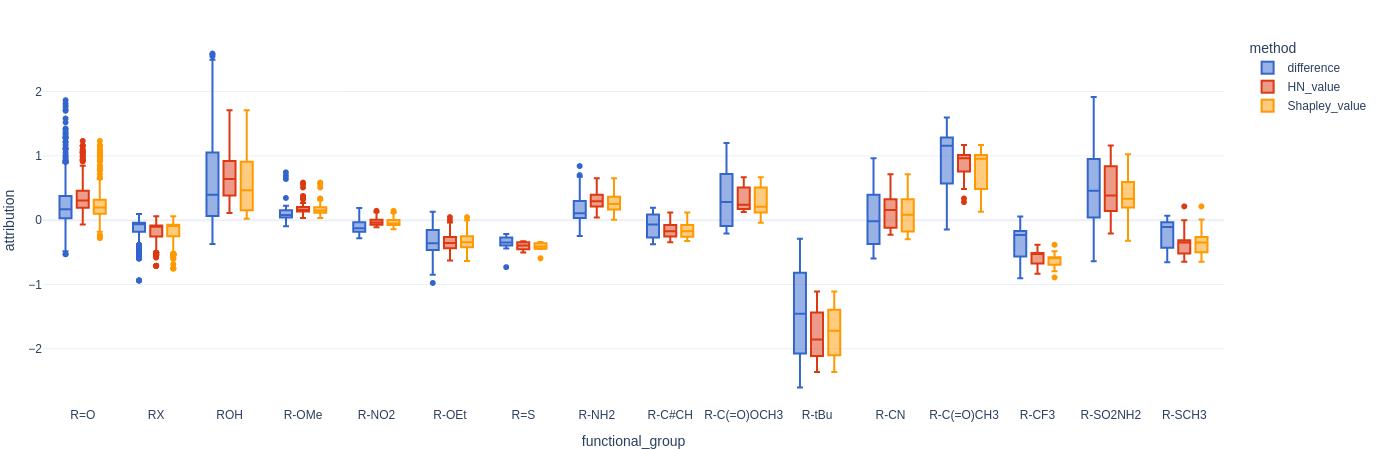
\includegraphics[scale=0.7]{../data/images/esol_attribution_distributions.png}
        \end{tikzfigure}

    }

    % Contact and Acknowledgements block.
    \block{Conclusions} {
        % Add the coclusions of your research.
    }

    % Block containing the references.
    \block{References} {
        \vspace{-1cm}
        \bibliography{poster.bib}
    }

    % Right Column.
    \column{0.5}

    % Theory
    \block{Theory}{
        % Add a small theory section. Keep your theory short and to the point.
    }

    % Results block 2.
    \block{}{
        % This is where you can add the rest of your results.

    }

    % Contact and Acknowledgements block.
    \block{Contact and acknowledgements} {
        Contact via email at xander.wieme@ugent.be. \\
        \begin{wrapfigure}[1]{r}{10cm}
            \vspace{-4cm}
            \begin{tikzfigure}[]
                
\includegraphics[height=4cm]{figures/ugent_logo}
            \end{tikzfigure}
        \end{wrapfigure}
    }


\end{columns}

\end{document}
